% A LaTeX template for MSc Thesis submissions to 
% Politecnico di Milano (PoliMi) - School of Industrial and Information Engineering
%
% Copyright 2021 Politecnico di Milano, Italy. NC-BY

\documentclass{Configuration_Files/PoliMi3i_thesis}

%------------------------------------------------------------------------------
%	REQUIRED PACKAGES AND  CONFIGURATIONS
%------------------------------------------------------------------------------

% CONFIGURATIONS
\usepackage{parskip} % For paragraph layout
\usepackage{setspace} % For using single or double spacing
\usepackage{emptypage} % To insert empty pages
\usepackage{minted}
\usepackage{multicol} % To write in multiple columns (executive summary)
\setlength\columnsep{15pt} % Column separation in executive summary
\setlength\parindent{0pt} % Indentation
\raggedbottom  


% PACKAGES FOR TITLES
\usepackage{titlesec}
% \titlespacing{\section}{left spacing}{before spacing}{after spacing}
\titlespacing{\section}{0pt}{3.3ex}{2ex}
\titlespacing{\subsection}{0pt}{3.3ex}{1.65ex}
\titlespacing{\subsubsection}{0pt}{3.3ex}{1ex}
\usepackage{color}

% PACKAGES FOR LANGUAGE AND FONT
\usepackage[english]{babel} % The document is in English  
\usepackage[utf8]{inputenc} % UTF8 encoding
\usepackage[T1]{fontenc} % Font encoding
\usepackage[11pt]{moresize} % Big fonts

% PACKAGES FOR IMAGES
\usepackage{graphicx}
\usepackage{transparent} % Enables transparent images
\usepackage{eso-pic} % For the background picture on the title page
\usepackage{subfig} % Numbered and caption subfigures using \subfloat.
\usepackage{tikz} % A package for high-quality hand-made figures.
\usetikzlibrary{}
\graphicspath{{./Images/}} % Directory of the images
\usepackage{caption} % Coloured captions
\usepackage{xcolor} % Coloured captions
\usepackage{amsthm,thmtools,xcolor} % Coloured "Theorem"
\usepackage{float}
\usepackage{hyperref}

% STANDARD MATH PACKAGES
\usepackage{amsmath}
\usepackage{amsthm}
\usepackage{amssymb}
\usepackage{amsfonts}
\usepackage{bm}
\usepackage[overload]{empheq} % For braced-style systems of equations.
\usepackage{fix-cm} % To override original LaTeX restrictions on sizes

% PACKAGES FOR TABLES
\usepackage{tabularx}
\usepackage{longtable} % Tables that can span several pages
\usepackage{colortbl}

% PACKAGES FOR ALGORITHMS (PSEUDO-CODE)
\usepackage{algorithm}
\usepackage{algorithmic}

% PACKAGES FOR REFERENCES & BIBLIOGRAPHY
\usepackage[colorlinks=true,linkcolor=black,anchorcolor=black,citecolor=black,filecolor=black,menucolor=black,runcolor=black,urlcolor=black]{hyperref} % Adds clickable links at references
\usepackage{cleveref}
\usepackage[square, numbers, sort&compress]{natbib} % Square brackets, citing references with numbers, citations sorted by appearance in the text and compressed
\bibliographystyle{abbrvnat} % You may use a different style adapted to your field

% OTHER PACKAGES
\usepackage{pdfpages} % To include a pdf file
\usepackage{afterpage}
\usepackage{lipsum} % DUMMY PACKAGE
\usepackage{fancyhdr} % For the headers
\fancyhf{}

% Input of configuration file. Do not change config.tex file unless you really know what you are doing. 
% Define blue color typical of polimi
\definecolor{bluepoli}{cmyk}{0.4,0.1,0,0.4}

% Custom theorem environments
\declaretheoremstyle[
  headfont=\color{bluepoli}\normalfont\bfseries,
  bodyfont=\color{black}\normalfont\itshape,
]{colored}

% Set-up caption colors
\captionsetup[figure]{labelfont={color=bluepoli}} % Set colour of the captions
\captionsetup[table]{labelfont={color=bluepoli}} % Set colour of the captions
\captionsetup[algorithm]{labelfont={color=bluepoli}} % Set colour of the captions

\theoremstyle{colored}
\newtheorem{theorem}{Theorem}[chapter]
\newtheorem{proposition}{Proposition}[chapter]

% Enhances the features of the standard "table" and "tabular" environments.
\newcommand\T{\rule{0pt}{2.6ex}}
\newcommand\B{\rule[-1.2ex]{0pt}{0pt}}

% Pseudo-code algorithm descriptions.
\newcounter{algsubstate}
\renewcommand{\thealgsubstate}{\alph{algsubstate}}
\newenvironment{algsubstates}
  {\setcounter{algsubstate}{0}%
   \renewcommand{\STATE}{%
     \stepcounter{algsubstate}%
     \Statex {\small\thealgsubstate:}\space}}
  {}

% New font size
\newcommand\numfontsize{\@setfontsize\Huge{200}{60}}

% Title format: chapter
\titleformat{\chapter}[hang]{
\fontsize{50}{20}\selectfont\bfseries\filright}{\textcolor{bluepoli} \thechapter\hsp\hspace{2mm}\textcolor{bluepoli}{|   }\hsp}{0pt}{\huge\bfseries \textcolor{bluepoli}
}

% Title format: section
\titleformat{\section}
{\color{bluepoli}\normalfont\Large\bfseries}
{\color{bluepoli}\thesection.}{1em}{}

% Title format: subsection
\titleformat{\subsection}
{\color{bluepoli}\normalfont\large\bfseries}
{\color{bluepoli}\thesubsection.}{1em}{}

% Title format: subsubsection
\titleformat{\subsubsection}
{\color{bluepoli}\normalfont\large\bfseries}
{\color{bluepoli}\thesubsubsection.}{1em}{}

% Shortening for setting no horizontal-spacing
\newcommand{\hsp}{\hspace{0pt}}

\makeatletter
% Renewcommand: cleardoublepage including the background pic
\renewcommand*\cleardoublepage{%
  \clearpage\if@twoside\ifodd\c@page\else
  \null
  \AddToShipoutPicture*{\BackgroundPic}
  \thispagestyle{empty}%
  \newpage
  \if@twocolumn\hbox{}\newpage\fi\fi\fi}
\makeatother

%For correctly numbering algorithms
\numberwithin{algorithm}{chapter}

%----------------------------------------------------------------------------
%	NEW COMMANDS DEFINED
%----------------------------------------------------------------------------

% EXAMPLES OF NEW COMMANDS
\newcommand{\bea}{\begin{eqnarray}} % Shortcut for equation arrays
\newcommand{\eea}{\end{eqnarray}}
\newcommand{\e}[1]{\times 10^{#1}}  % Powers of 10 notation

%----------------------------------------------------------------------------
%	ADD YOUR PACKAGES (be careful of package interaction)
%----------------------------------------------------------------------------

%----------------------------------------------------------------------------
%	ADD YOUR DEFINITIONS AND COMMANDS (be careful of existing commands)
%----------------------------------------------------------------------------

%----------------------------------------------------------------------------
%	BEGIN OF YOUR DOCUMENT
%----------------------------------------------------------------------------

\begin{document}

\fancypagestyle{plain}{%
\fancyhf{} % Clear all header and footer fields
\fancyhead[RO,RE]{\thepage} %RO=right odd, RE=right even
\renewcommand{\headrulewidth}{0pt}
\renewcommand{\footrulewidth}{0pt}}

%----------------------------------------------------------------------------
%	TITLE PAGE
%----------------------------------------------------------------------------

\pagestyle{empty} % No page numbers
\frontmatter % Use roman page numbering style (i, ii, iii, iv...) for the preamble pages

\puttitle{
	title=Systems and Methods for Big and Unstructured Data Project,
	name1=Angelo Prete,
	name2=Antonio Riverso, 
	name3=Andrea Sanvito,
	academicyear=2024-2025,
	groupnumber=32
} % These info will be put into your Title page 

%----------------------------------------------------------------------------
%	PREAMBLE PAGES: ABSTRACT (inglese e italiano), EXECUTIVE SUMMARY
%----------------------------------------------------------------------------
\startpreamble
\setcounter{page}{1} % Set page counter to 1

%----------------------------------------------------------------------------
%	LIST OF CONTENTS/FIGURES/TABLES/SYMBOLS
%----------------------------------------------------------------------------

% TABLE OF CONTENTS
\thispagestyle{empty}
\tableofcontents % Table of contents 
\thispagestyle{empty}
\cleardoublepage

%-------------------------------------------------------------------------
%	THESIS MAIN TEXT
%-------------------------------------------------------------------------
% In the main text of your thesis you can write the chapters in two different ways:
%
%(1) As presented in this template you can write:
%    \chapter{Title of the chapter}
%    *body of the chapter*
%
%(2) You can write your chapter in a separated .tex file and then include it in the main file with the following command:
%    \chapter{Title of the chapter}
%    \input{chapter_file.tex}
%
% Especially for long thesis, we recommend you the second option.

\addtocontents{toc}{\vspace{2em}} % Add a gap in the Contents, for aesthetics
\mainmatter % Begin numeric (1,2,3...) page numbering

\chapter{Introduction}

For the project, we decided to analyze two datasets, the Formula 1 dataset and the Letterboxd dataset. Both of them can be found at Kaggle.

\section{Letterbox Database}

Our first analysis is on the \href{https://www.kaggle.com/datasets/gsimonx37/letterboxd}{Letterboxd Movies Dataset}, that is a comprehensive collection of movie-related data derived from the \href{https://letterboxd.com/}{Letterboxd} website. It contains information about movies, such as titles, release dates, genres, average ratings, directors, actors, studios, and production details.

The raw dataset was cleaned and processed using a Python script. This script replaced unsupported characters in the CSV files to ensure compatibility with the database. After cleaning, we imported the dataset into a Neo4j database, creating nodes for movies, actors, genres, and studios, and establishing relationships like actors starring in movies and genres linked to films.

We decided to use Neo4j since it makes the process of querying connected data like movies, actors and directors simple. The queries rely heavily on relationships—such as finding actor-director pairings or tracking genre trends over time—and Neo4j is designed to navigate these links efficiently. Since it is schema-free handling data like ours with a lot of missing values becomes easier. Additionally, importing and linking data from CSV files is very straightforward.

\chapter{Data Wrangling}
\section{Letterbox dataset data wrangling}
In order to ensure clean and consistent CSV data for import into Neo4j, we performed 
a small data wrangling step in Python by using the following function. This step replaced any irregular escaped quotes 
(e.g. \texttt{\textbackslash \"}) in our raw CSV files with standard quotes, preventing 
errors during loading.

\subsection*{Python Script for Cleaning CSV Files}

\inputminted{python}{letterboxd/letterboxdDataCleaning.py}

\chapter{Dataset}

\section{Letterbox dataset}

As stated in the dataset page on Kaggle, the dataset is provided through csv files with the following structure:

\begin{itemize}
    \item \textbf{movies.csv} - Basic information about films:
    \begin{itemize}
        \item \textit{id} - Movie identifier (primary key);
        \item \textit{name} - The name of the film;
        \item \textit{date} - Year of release of the film;
        \item \textit{tagline} - The slogan of the film;
        \item \textit{description} - Description of the film;
        \item \textit{minute} - Movie duration (in minutes);
        \item \textit{rating} - Average rating of the film.
    \end{itemize}
    \item \textbf{actors.csv} - Actors who took part in the filming of films:
    \begin{itemize}
        \item \textit{id} - Movie identifier (foreign key);
        \item \textit{name} - Name;
        \item \textit{role} - Role.
    \end{itemize}
    \item \textbf{crew.csv} - Film crew:
    \begin{itemize}
        \item \textit{id} - Movie identifier (foreign key);
        \item \textit{role} - Role in the film crew (director, screenwriter, etc.);
        \item \textit{name} - Name.
    \end{itemize}
    \item \textbf{languages.csv} - In what languages the films were shot:
    \begin{itemize}
        \item \textit{id} - Movie identifier (foreign key);
        \item \textit{type} - Type (primary, conversational, etc.);
        \item \textit{language} - Film language.
    \end{itemize}
    \item \textbf{studios.csv} - Film studios:
    \begin{itemize}
        \item \textit{id} - Movie identifier (foreign key);
        \item \textit{studio} - Film studio.
    \end{itemize}
    \item \textbf{countries.csv} - Countries:
    \begin{itemize}
        \item \textit{id} - Movie identifier (foreign key);
        \item \textit{country} - Country.
    \end{itemize}
    \item \textbf{genres.csv} - Film genres:
    \begin{itemize}
        \item \textit{id} - Movie identifier (foreign key);
        \item \textit{genre} - Film genre.
    \end{itemize}
    \item \textbf{themes.csv} - Themes in films:
    \begin{itemize}
        \item \textit{id} - Movie identifier (foreign key);
        \item \textit{theme} - The theme of the film.
    \end{itemize}
    \item \textbf{releases.csv} - Movie releases:
    \begin{itemize}
        \item \textit{id} - Movie identifier (foreign key);
        \item \textit{country} - Release country;
        \item \textit{date} - Release date of the film;
        \item \textit{type} - Release type (theatrical, television, etc.) of the film;
        \item \textit{rating} - Age rating of the film.
    \end{itemize}
    \item \textbf{posters.csv} - Movie posters:
    \begin{itemize}
        \item \textit{id} - Movie identifier (foreign key);
        \item \textit{country} - URL address.
    \end{itemize}
\end{itemize}

Since we don't need the posters for our analysis, we didn't import it in our Neo4j instance.

The other files were imported using the following commands (through peridic commits, given their sizes):

\inputminted[frame=single,framesep=10pt,breaklines]{cypher}{letterboxd/import/movies.cypher}
\inputminted[frame=single,framesep=10pt,breaklines]{cypher}{letterboxd/import/actors.cypher}
\inputminted[frame=single,framesep=10pt,breaklines]{cypher}{letterboxd/import/crew.cypher}
\inputminted[frame=single,framesep=10pt,breaklines]{cypher}{letterboxd/import/languages.cypher}
\inputminted[frame=single,framesep=10pt,breaklines]{cypher}{letterboxd/import/studio.cypher}
\inputminted[frame=single,framesep=10pt,breaklines]{cypher}{letterboxd/import/country.cypher}
\inputminted[frame=single,framesep=10pt,breaklines]{cypher}{letterboxd/import/genre.cypher}
\inputminted[frame=single,framesep=10pt,breaklines]{cypher}{letterboxd/import/theme.cypher}
\inputminted[frame=single,framesep=10pt,breaklines]{cypher}{letterboxd/import/release.cypher}

An example of the produced structure can be seen in figure \ref{fig:graph_example}, where we show some nodes (one of each type present in the database) related to the movie "The Wolf of Wall Street".
\begin{figure}[!h]
    \centering
    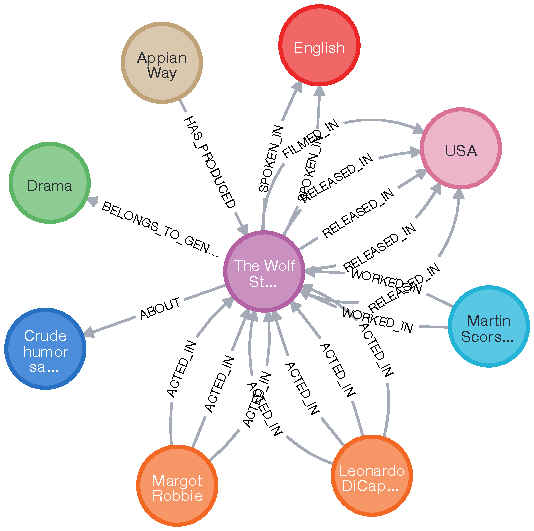
\includegraphics[width=0.6\linewidth]{Project Template/letterboxd/graph_example.pdf}
    \caption{Truncated graph of "The Wolf of Wall Street" movie}
    \label{fig:graph_example}
\end{figure}

\chapter{Queries}

\section{Letterbox dataset queries}

\subsection{Average rating, length and number of movies over the years}

With this query we calculated the average rating, duration, and number of movies released each year for films over 60 minutes, excluding those from 2024 (since the dataset is incomplete for the year). It helped us identify trends in movie quality and length over time, plotted in the graphs below.

\inputminted[frame=single,framesep=10pt,breaklines]{cypher}{letterboxd/queries/query1.cypher}

The query returns the following (truncated) result:

\begin{table}[h!]
\centering
\begin{tabular}{|c|c|c|c|}
\hline
\textbf{YEAR} & \textbf{AVG\_RATING} & \textbf{AVG\_DURATION} & \textbf{N\_MOVIES} \\ \hline
2023 & 3.18 & 121.77 & 15598 \\ \hline
2022 & 3.15 & 125.01 & 14869 \\ \hline
2021 & 3.17 & 122.92 & 13841 \\ \hline
2020 & 3.15 & 120.36 & 12372 \\ \hline
2019 & 3.16 & 114.06 & 14173 \\ \hline
2018 & 3.14 & 112.90 & 13473 \\ \hline
2017 & 3.14 & 111.82 & 12963 \\ \hline
\end{tabular}
\caption{Average Rating, Duration, and Number of Movies by Year}
\end{table}

\begin{figure}[!h]
  \centering
  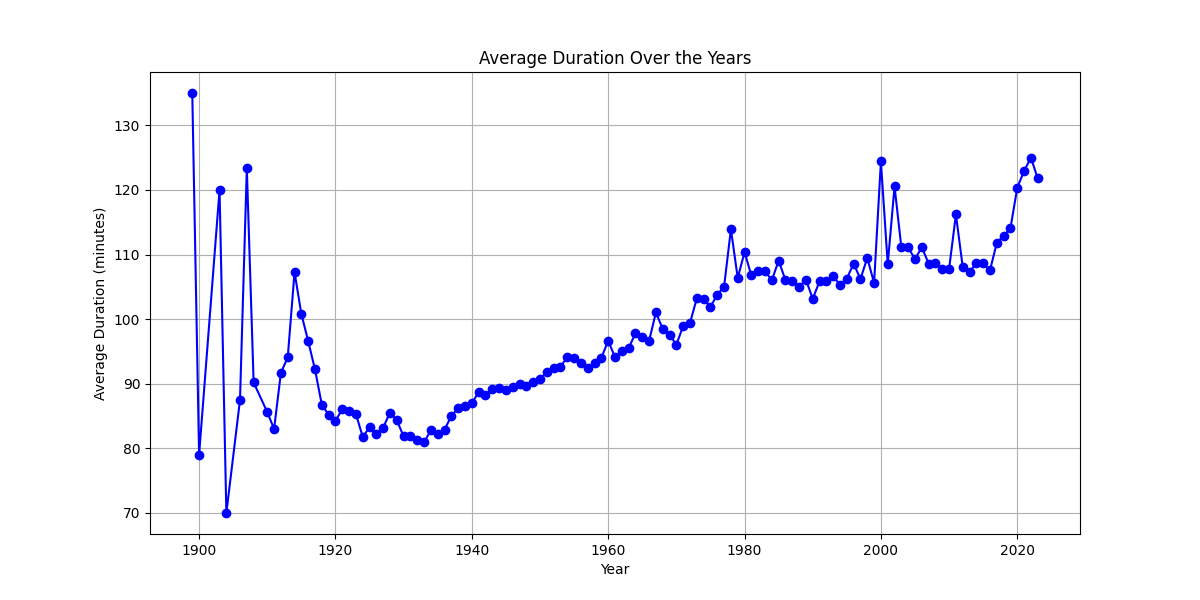
\includegraphics[width=\textwidth]{Project Template/letterboxd/visualization/average_duration_trend.png}
  \caption{Average movie duration trend.}
  \label{fig:duration_trend}
\end{figure}

\begin{figure}[!h]
  \centering
  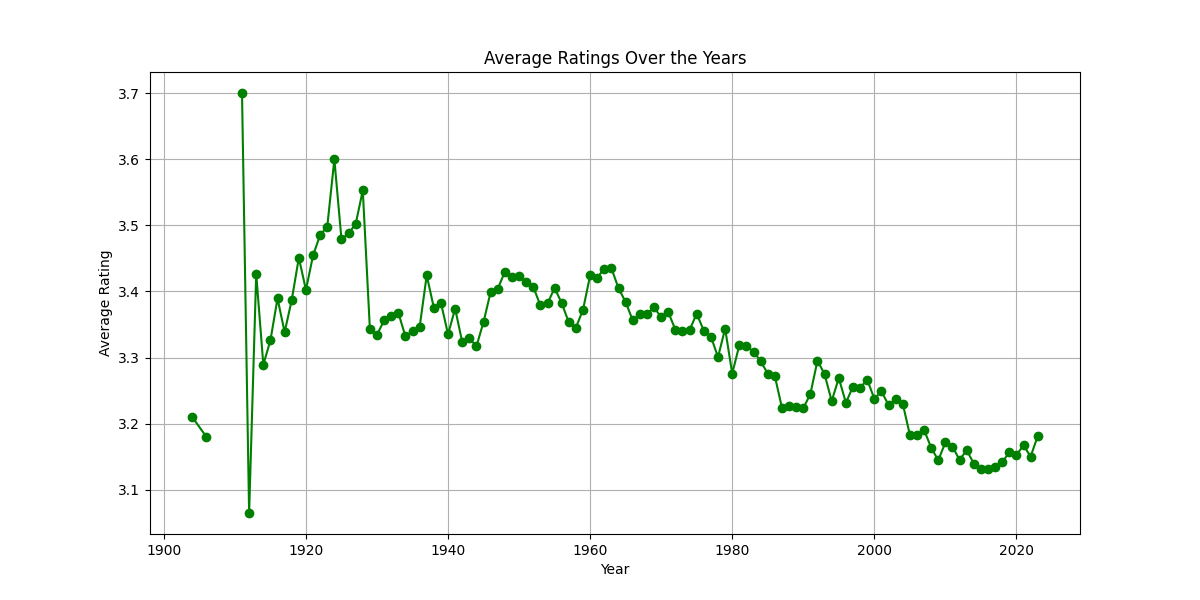
\includegraphics[width=\textwidth]{Project Template/letterboxd/visualization/average_ratings_trend.png}
  \caption{Average movie ratings trend.}
  \label{fig:ratings_trend}
\end{figure}

\begin{figure}[!h]
  \centering
  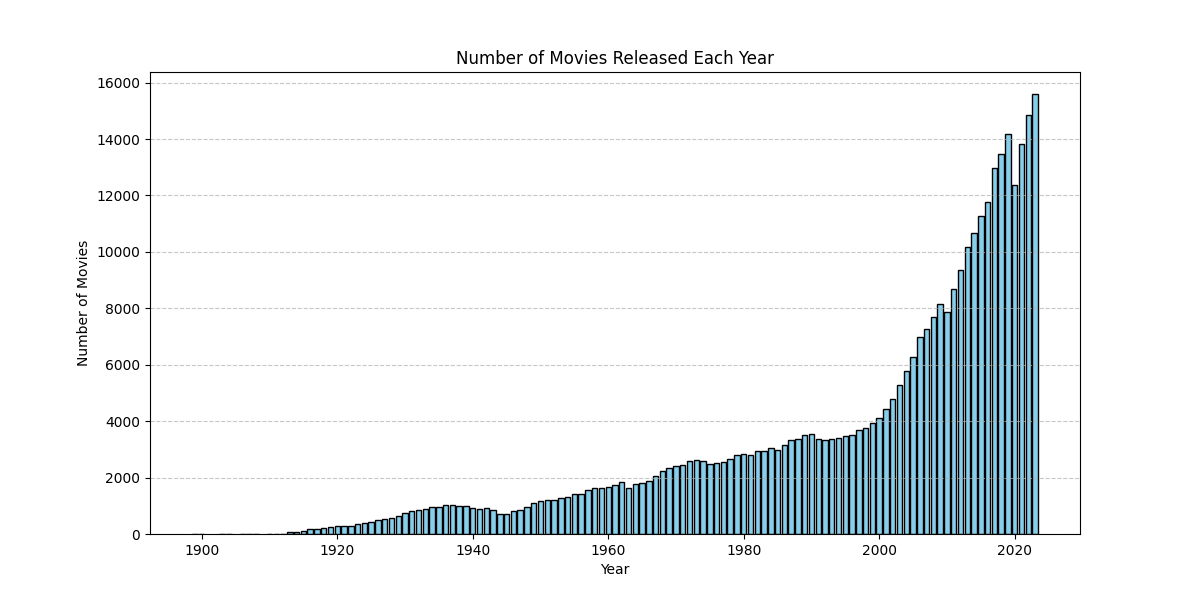
\includegraphics[width=\textwidth]{Project Template/letterboxd/visualization/movies_count_trend.png}
  \caption{Movies count trend.}
  \label{fig:movies_count_trend}
\end{figure}


\subsection{Most consistent directors (all movies with high ratings)}

This query returns the list of directors found to be more consistent w.r.t the rating of their movies. To do it we used a scoring function (inspired to the tf-idf one) that multiplies the average rating of all movies by the logarithm (applied twice in this case) of their number.

\inputminted[frame=single,framesep=10pt,breaklines]{cypher}{letterboxd/queries/query2.cypher}

The query returns the following (truncated) result:

\begin{longtable}{|c|l|c|c|}[!h]
\caption{Most consistent directors} \\
\hline
\# & Director & Avg. Rating & Number of Movies \\
\hline
\endfirsthead
\hline
\# & Director & Avg. Rating & Number of Movies \\
\hline
\endhead
\hline
\endfoot
\hline
\endlastfoot

1 & Chuck Jones        & 3.47 & 223 \\
2 & Friz Freleng       & 3.37 & 184 \\
3 & William Hanna      & 3.50 & 124 \\
4 & Joseph Barbera     & 3.50 & 123 \\
5 & Jean-Luc Godard    & 3.54 & 105 \\
6 & Tex Avery          & 3.43 & 108 \\
7 & Dave Fleischer     & 3.43 & 104 \\
8 & Georges Méliès     & 3.20 & 173 \\
9 & Stan Brakhage      & 3.50 & 88  \\
10 & Agnès Varda       & 3.75 & 54  \\
11 & Martin Scorsese   & 3.74 & 54  \\
12 & Ingmar Bergman    & 3.67 & 60  \\
13 & Werner Herzog     & 3.57 & 66  \\
14 & John Ford         & 3.50 & 71  \\
15 & Krzysztof Kieślowski & 3.74 & 44  \\
\end{longtable}

\subsection{Average rating by genre}

We wrote this query because we where interested in finding which genres had better reviewed movies by users on Letterboxd. Having an higher score doesn't necessarily mean that the movies of that category are better, it could alse be that the users of the platform like the genre more.
As we expected, the horror genre is the one populated by low quality movies.

\inputminted[frame=single,framesep=10pt,breaklines]{cypher}{letterboxd/queries/query3.cypher}

The query returns the following result:

\begin{longtable}[!h]{|c|l|c|}
\caption{Genre average ratings} \\
\hline
\# & Genre & Rating \\
\hline
\endfirsthead
\hline
\# & Genre & Rating \\
\hline
\endhead
\hline
\endfoot
\hline
\endlastfoot
1 & Documentary       & 3.52 \\
2 & Music             & 3.44 \\
3 & History           & 3.40 \\
4 & War               & 3.38 \\
5 & Animation         & 3.36 \\
6 & Drama             & 3.33 \\
7 & Western           & 3.29 \\
8 & Crime             & 3.24 \\
9 & Romance           & 3.19 \\
10 & Comedy            & 3.18 \\
11 & Mystery           & 3.18 \\
12 & Fantasy           & 3.15 \\
13 & TV Movie          & 3.11 \\
14 & Family            & 3.11 \\
15 & Adventure         & 3.10 \\
16 & Action            & 3.05 \\
17 & Thriller          & 3.05 \\
18 & Science Fiction   & 3.03 \\
19 & Horror            & 2.92 \\
\end{longtable}

\begin{figure}[!h]
  \centering
  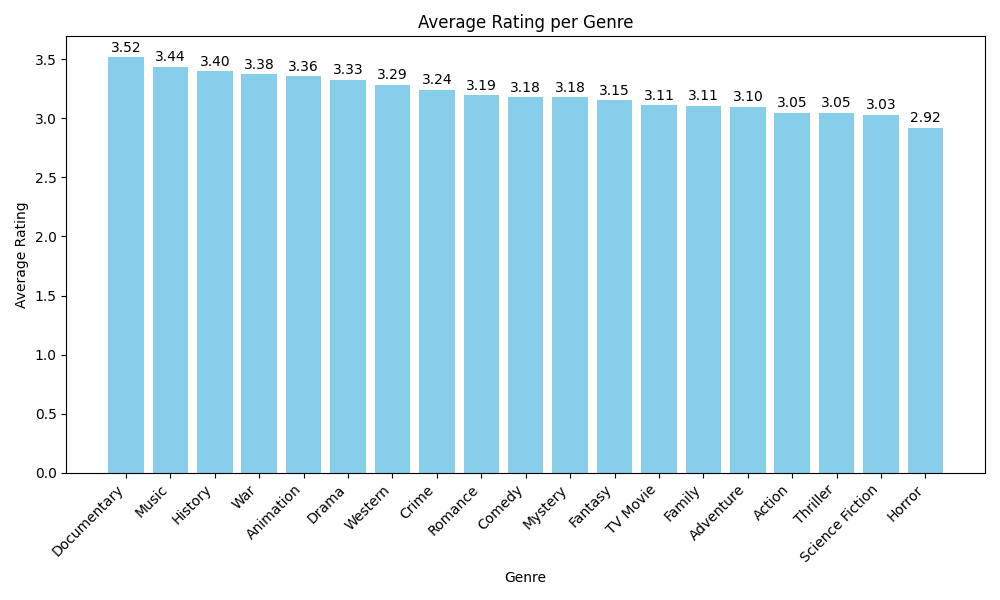
\includegraphics[width=\textwidth]{Project Template/letterboxd/visualization/average_rating_genre.png}
  \caption{Average rating for genre.}
  \label{fig:average_rating_genre}
\end{figure}

\subsection{Most Productive Studios by Year}

With this query we found the most productive movie studios by year between 1900 and 2023, considering only movies with a rating of 3 or higher (i.e. at least 6/10). The query calculates the number of qualifying movies produced by each studio for each year, returning the year, studio name, and count of movies.
We decided to stop at 5 studios for each year.

\inputminted[frame=single,framesep=10pt,breaklines]{cypher}{letterboxd/queries/query4.cypher}

The query returns the following (truncated to include only 2022 and 2034) result:

\begin{longtable}[!h]{|c|l|c|}
\caption{Top Studios through years by movie count} \\
\hline
Year & Studio & Movies Count \\
\hline
\endfirsthead
\hline
Year & Studio & Movies Count \\
\hline
\endhead
\hline
\endfoot
\hline
\endlastfoot

2023 & France 2 Cinéma & 32 \\
2023 & HBO Documentary Films & 31 \\
2023 & Amazon Studios & 29 \\
2023 & RAI Cinema & 28 \\
2023 & France 3 Cinéma & 27 \\
2022 & ARTE & 38 \\
2022 & France 2 Cinéma & 30 \\
2022 & Amazon Studios & 24 \\
2022 & RAI Cinema & 21 \\
2022 & ARTE France Cinéma & 20 \\

\end{longtable}

\subsection{Genre popularity through the years}

While this query might look simple, it highlights how genres alternated through the years in popularity. It shows how in recent years, while drama has always been a relevant genre, comedy and documentaries have rose in popularity.

\inputminted[frame=single,framesep=10pt,breaklines]{cypher}{letterboxd/queries/query5.cypher}

The output of this query has been truncated to show genre popularity only of 2022 and 2023:

\begin{longtable}[!h]{|c|l|c|}
\caption{Genre popularity through the years} \\
\hline
\textbf{Year} & \textbf{Genre} & \textbf{Count} \\
\hline
\endfirsthead
\hline
\textbf{Year} & \textbf{Genre} & \textbf{Count} \\
\hline
\endhead
\hline
\endfoot
\hline
2023 & Drama & 1423 \\
2023 & Comedy & 751 \\
2023 & Documentary & 557 \\
2023 & Thriller & 263 \\
2023 & Crime & 256 \\
2023 & Animation & 236 \\
2023 & Romance & 233 \\
2023 & Action & 174 \\
2023 & Mystery & 155 \\
2023 & Horror & 153 \\
2023 & Music & 128 \\
2023 & Family & 121 \\
2023 & Science Fiction & 106 \\
2023 & Fantasy & 103 \\
2023 & History & 102 \\
2023 & Adventure & 97 \\
2023 & TV Movie & 64 \\
2023 & War & 40 \\
2023 & Western & 10 \\
2022 & Drama & 1445 \\
2022 & Comedy & 792 \\
2022 & Documentary & 642 \\
2022 & Thriller & 280 \\
2022 & Animation & 266 \\
2022 & Romance & 263 \\
2022 & Crime & 241 \\
2022 & Horror & 199 \\
2022 & Mystery & 183 \\
2022 & Music & 164 \\
2022 & Action & 149 \\
2022 & Fantasy & 135 \\
2022 & Science Fiction & 120 \\
2022 & History & 119 \\
2022 & Family & 105 \\
2022 & Adventure & 92 \\
2022 & TV Movie & 78 \\
2022 & War & 39 \\
2022 & Western & 7 \\
\end{longtable}


\begin{figure}[!h]
  \centering
  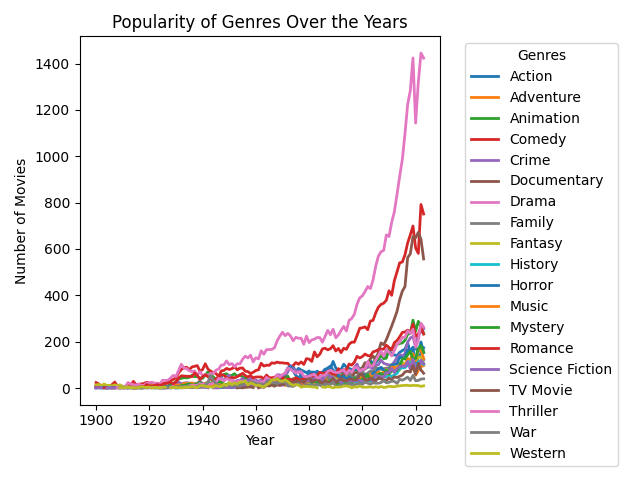
\includegraphics[width=\textwidth]{Project Template/letterboxd/visualization/genre_popularity.png}
  \caption{Genre popularity through the years.}
  \label{fig:genre_popularity}
\end{figure}

\subsection{Actors who acted in highly rated movies}

Here, we wanted to see which actors (who acted in at least 20 movies) took part in movies that are highly rated since 2000. The list of names is quite recognizable, as you will see.

\inputminted[frame=single,framesep=10pt,breaklines]{cypher}{letterboxd/queries/query6.cypher}

\begin{table}
\centering
\begin{tabular}[h!]{|l|c|c|}
\hline
\textbf{Actor} & \textbf{Rating} & \textbf{Count} \\
\hline
Viggo Mortensen & 3.8034 & 21 \\
Leonardo DiCaprio & 3.7725 & 24 \\
Jorma Taccone & 3.6316 & 21 \\
Lucas Hedges & 3.6232 & 21 \\
Mahershala Ali & 3.6213 & 21 \\
Ryan Gosling & 3.6192 & 30 \\
Jason Schwartzman & 3.6172 & 52 \\
Tilda Swinton & 3.6001 & 42 \\
Tobey Maguire & 3.5895 & 22 \\
Cillian Murphy & 3.5873 & 25 \\
Frank Wood & 3.5785 & 23 \\
Maggie Gyllenhaal & 3.5754 & 28 \\
Caleb Landry Jones & 3.5451 & 25 \\
Joaquin Phoenix & 3.5387 & 30 \\
Dave Chappelle & 3.5353 & 23 \\
Andy Serkis & 3.5336 & 33 \\
Sherry Lynn & 3.5309 & 21 \\
Timothée Chalamet & 3.5299 & 27 \\
Paul Dano & 3.5231 & 36 \\
\hline
\end{tabular}
\caption{Actor who acted in highly rated movies}
\end{table}

\subsection{Number of good movies by years and by  countries they were filmed in}

\inputminted[frame=single,framesep=10pt,breaklines]{cypher}{letterboxd/queries/query7.cypher}

\begin{figure}[!h]
  \centering
  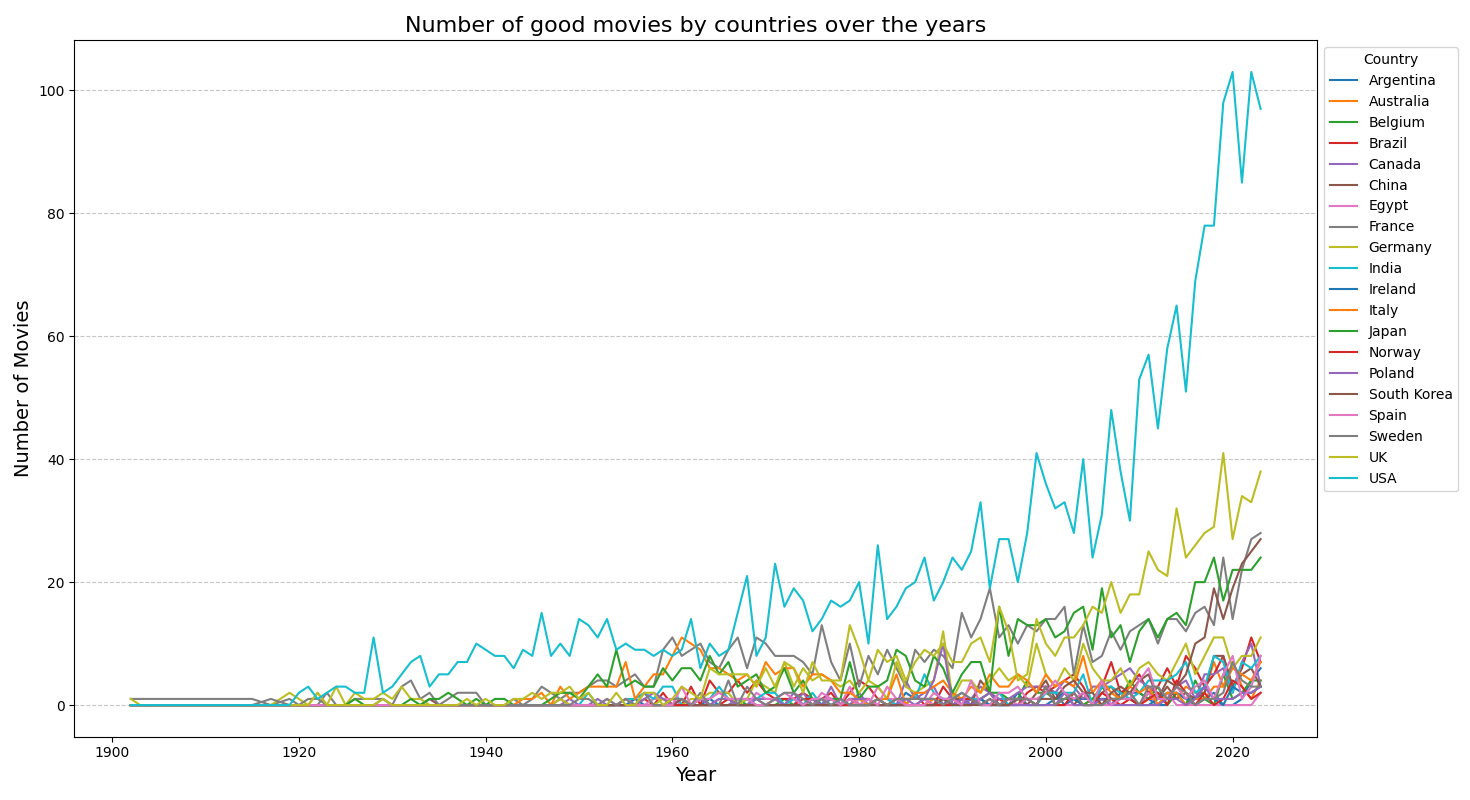
\includegraphics[width=\textwidth]{Project Template/letterboxd/visualization/good_movies_by_country.png}
  \caption{Digital vs Theatrical releases.}
  \label{fig:good_movies_by_countries}
\end{figure}
\subsection{Frequent actor-genre pairings (since 2000)}

Most actors often star in movies of the same genre, so we wanted to find the ones that are particularly "loyal" to a certain genre. To do it we used the following query:

\inputminted[frame=single,framesep=10pt,breaklines]{cypher}{letterboxd/queries/query8.cypher}

This is the truncated output with the first 20 pairings:

\begin{table}[!h]
\centering
\begin{tabular}{|l|l|r|}
\hline
\textbf{Actor} & \textbf{Genre} & \textbf{Appearances} \\
\hline
Dave Bautista & Science Fiction & 119 \\
Willem Dafoe & Drama & 110 \\
Benedict Cumberbatch & Drama & 108 \\
Joseph Oliveira & Drama & 105 \\
Dave Bautista & Adventure & 104 \\
Brad Pitt & Drama & 102 \\
Timothée Chalamet & Drama & 98 \\
Samuel L. Jackson & Action & 90 \\
Leonardo DiCaprio & Drama & 89 \\
Willem Dafoe & Comedy & 86 \\
Mark Ruffalo & Drama & 81 \\
Stan Lee & Action & 80 \\
Mark Ruffalo & Science Fiction & 80 \\
Tilda Swinton & Drama & 79 \\
Samuel L. Jackson & Adventure & 78 \\
Stan Lee & Adventure & 74 \\
Josh Brolin & Adventure & 72 \\
Dave Bautista & Action & 72 \\
J.K. Simmons & Science Fiction & 70 \\
\hline
\end{tabular}
\caption{Actor-Genre pairings}
\end{table}

\subsection{Frequent actor-director pairings in movies with good ratings and produced in USA
}

The original idea behind this query was to find all pairings actor-director, but since the dataset was too big to do so (even with the help of indexes), we decided to restrict the query to include only pairings in movies produced since 2000 in USA.

\inputminted[frame=single,framesep=10pt,breaklines]{cypher}{letterboxd/queries/query9.cypher}

Some of the results we found were expected, like Samuel L. Jackson and Tarantino or DiCaprio and Scoresese; the other top 20 pairings are in the following table:

\begin{table}[h!]
\centering
\begin{tabular}{|l|l|r|}
\hline
\textbf{Actor} & \textbf{Director} & \textbf{Count} \\
\hline
Michael Caine & Christopher Nolan & 187 \\
Samuel L. Jackson & Quentin Tarantino & 173 \\
Quentin Tarantino & Quentin Tarantino & 170 \\
Mel Blanc & Chuck Jones & 161 \\
Cillian Murphy & Christopher Nolan & 159 \\
Willem Dafoe & Wes Anderson & 130 \\
Leonardo DiCaprio & Martin Scorsese & 126 \\
Dave Bautista & James Gunn & 120 \\
Joseph Oliveira & Christopher Nolan & 112 \\
Samuel L. Jackson & Joe Russo & 102 \\
Samuel L. Jackson & Anthony Russo & 102 \\
Chris Evans & Joe Russo & 96 \\
Sebastian Stan & Joe Russo & 96 \\
Dave Bautista & Joe Russo & 96 \\
Chris Evans & Anthony Russo & 96 \\
Sebastian Stan & Anthony Russo & 96 \\
Dave Bautista & Anthony Russo & 96 \\
Dave Bautista & Denis Villeneuve & 94 \\
Jason Schwartzman & Wes Anderson & 92 \\
\hline
\end{tabular}
\caption{Actor-director pairings}
\end{table}

 \subsection{Theatrical vs Digital releases}

 For the last query, we wanted to see how movie releases changed since the introduction of online renting and streaming.

 \inputminted[frame=single,framesep=10pt,breaklines]{cypher}{letterboxd/queries/query10.cypher}

 \begin{table}[!h]
\centering
\begin{tabular}{|r|l|r|}
\hline
\textbf{Release Year} & \textbf{Release Type} & \textbf{Total Movies} \\
\hline
2023 & Theatrical & 12161 \\
2023 & Digital & 11671 \\
2022 & Digital & 11033 \\
2022 & Theatrical & 10984 \\
2021 & Digital & 12381 \\
2021 & Theatrical & 10072 \\
2020 & Digital & 12645 \\
2020 & Theatrical & 9466 \\
2019 & Theatrical & 12323 \\
2019 & Digital & 7174 \\
2018 & Theatrical & 12629 \\
2018 & Digital & 5766 \\
\hline
\end{tabular}
\caption{Release Year, Release Type, and Total Movies}
\end{table}

 By looking at the graph we generated from the query result1, we can notice how during Covid digital releases overtook theatrical ones (as expected) and, more in general, how digital releases have been on the rise since early 2000s.

\begin{figure}[!h]
  \centering
  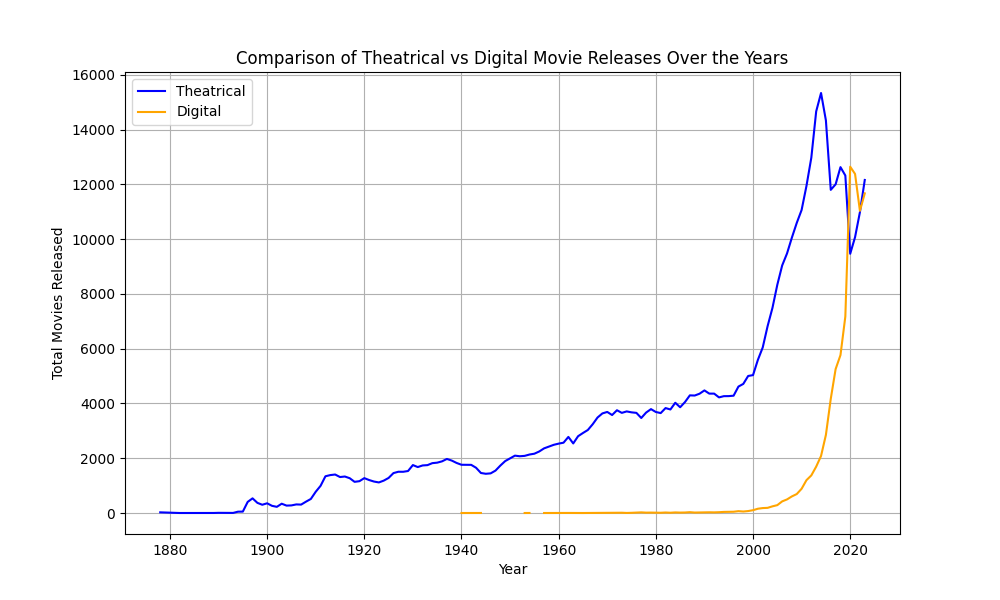
\includegraphics[width=\textwidth]{Project Template/letterboxd/visualization/releases.png}
  \caption{Digital vs Theatrical releases.}
  \label{fig:releases}
\end{figure}


%-------------------------------------------------------------------------
%	APPENDICES
%-------------------------------------------------------------------------

% \cleardoublepage
% \addtocontents{toc}{\vspace{2em}} % Add a gap in the Contents, for aesthetics
% \appendix
% \chapter{Appendix A}
% If you need to include an appendix to support the research in your thesis, you can place it at the end of the manuscript.
% An appendix contains supplementary material (figures, tables, data, codes, mathematical proofs, surveys, \dots)
% which supplement the main results contained in the previous chapters.


% % LIST OF FIGURES
\listoffigures

% % LIST OF TABLES
\listoftables

\cleardoublepage

\end{document}
